\chapter{System Design}
\section{Overview}
\paragraph{} This chapter describes the overall design of the wireless communicated robot movement and the web application working for the live feed from camera mounted on the robot. As we already know the hardware and software components used we will further go ahead and discuss the system design that we developed.
\section{Designing the Web Application}
\paragraph{}Web technologies we are using for the project are HTML, CSS, Bootstrap, Python and Flask. These technologies are needed to configured in a proper manner for the web application to work properly. In the directory where the project folder for the web application is established all the constituent files and folders have to be kept in a specific format as supported by Flask.

\begin{figure}[h]
\centering
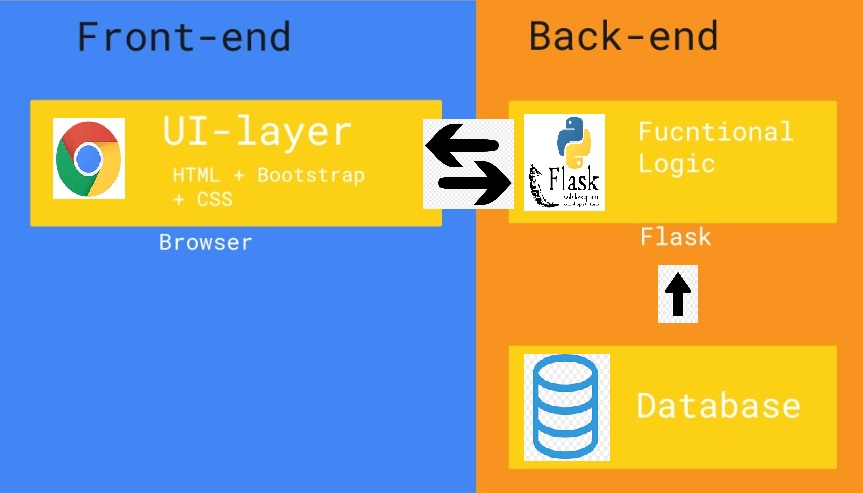
\includegraphics[scale=0.4]{bdweb.jpg}
\caption{Block Diagram of Web Application}
\end{figure}

\subsubsection*{Here is the basic file structure for flask:} 
\texttt{\textbf{\small{yourapp/}}}

\texttt{\small{.py}}

\textbf{\texttt{\small{static/}}}

\hspace{0.5in}\texttt{\small{.js}}

\hspace{0.5in}\texttt{\small{.css}}

\hspace{0.5in}\texttt{\small{Images}}

\textbf{\texttt{\small{templates/}}}

\hspace{0.5in}\texttt{\small{.html}}

\subsubsection*{Description of files:}
\textbf{.py}: contains the actual python code that will import the app
and start the \\development server.\\
\textbf{static/} : contains static files i.e. CSS (including bootstrap), JavaScript, images.\\
\textbf{templates/} : This is where you store your HTML templates
i.e. index.html, \\layout.html\\
Python modules used in app.py (main web app Script/Program):
\begin{enumerate}[1.]
\item Flask - Web application framework
\item CV2 - Library to help the drawing process with Open-CV
\item Sockets - provides access to the BSD socket interface
\item Keyboard - provides various keys-related functions
\item Time - provides various time-related functions
\item Rpi.GPIO - This package provides a class to control the GPIO on a Raspberry Pi.
\end{enumerate}

\section{Designing the remote controlled robot movement}
The heart of the robot is a raspberry pi 4(2GB RAM) which is a credit card sized computer used in a wide range of applications varying from a simple personal \\computer to advanced robotics.  The raspberry pi has an inbuilt Wi-Fi module which can connect to any network. The OS of the raspberry pi resides within an SD card of size 32 GB. The motors of the robot are controlled using the PWM pins available on the 40 pin GPIOS of the raspberry pi. The raspberry pi GPIO pins output a \\current insufficient to drive the motors and hence we have used the L298N motor driver which amplifies the current so that it drives the motors easily. In order to get \\information about the surroundings of the area in which the robot is patrolling we have used three sensors. They are ultrasonic sensors, Picamera v2.1 and a USB mic. The ultrasonic sensor is used to measure distances on all sides of the robot in order to ensure that the robot doesn’t collide with any obstacles in its vicinity. The Picamera acts as the eyes of the robot. The robot is steered using the ‘a’, ’w’, ‘s’ and ‘d’ keys of the robot based on the camera feed received. The USB mic acts like the ears of the robot. Using the mic, the robot can capture audio within its vicinity.
\begin{figure}[h]
\centering
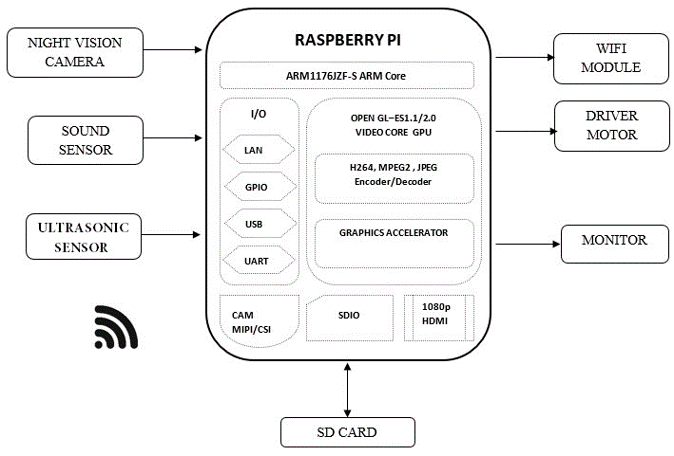
\includegraphics[scale=0.8]{bdrobot.png}
\caption{Block Diagram of Robot}
\end{figure}
\subsection{TCP/IP Communication}
The communication protocol which we have opted to use in our project is the TCP/IP socket protocol.  The TCP/IP socket protocol establishes a peer-to-peer connection between the server and the client followed by which data is transferred in the form of packets of fixed length. In our case each packet is 1024 bytes in length. A socket is one end of a 2-way communication. A socket consists of an IPV4 address and a port number. The connection between the server and the client happens with a series of events occurring on both the server and the client sides.
\subsubsection*{The following occurs on the server side:} 
\begin{enumerate}[1.]
\item Declaration of the socket object: first a socket object is created which is an \\instance of the socket class.
\item Socket binding: The process of assigning a port number to a socket is called socket binding.  
\item Listening for connections: Once the socket has been binded it soon starts listening for connection requests from active clients. 
\item Accepting Client connections: The server accepts all the client connections who are willing to connect to the server. Upon connection the server receives \\connection objects using which the server sends data to the client.
\item Data transfer: The server uses the connection objects to send data to the client.
\end{enumerate}
\subsubsection*{The following occurs on the client side:}
\begin{enumerate}[1.]
\item Declaration of the socket object: first a socket object is created which is an \\instance of the socket class.
\item Connection: The client sends a connection request to the server using the ip and port number of the server. 
\item Data transfer: Once the server accepts the connection of the client, the client starts receiving the data sent by the server.
\end{enumerate}
\subsection{GIX algorithm}
The GIX algorithm is an acronym for “Gone in exchange” Algorithm . The GIX algorithm ensures that data is transferred securely over the internet by using \\encryption and decryption algorithms on the sender and the receiver sides \\respectively.
\subsubsection*{The following occurs on the sender side: }
\begin{enumerate}
\item First the pure control message is received. Which in our case is the key pressed.
\item A random key is chosen and the control message is encrypted using the key.
\item The random key is hidden within the encrypted control message and the final encrypted message is returned.
\item The encrypted message is sent over the internet.
\end{enumerate}
\subsubsection*{The following occurs on the receiver side: }
\begin{enumerate}
\item The encrypted control message is received. 
\item The hidden key is found within the encrypted message.
\item Using the key, the message is decrypted to get the pure control message.
\item Appropriate tasks are performed based on the control message received. 
\end{enumerate}
\begin{figure}[h]
\centering
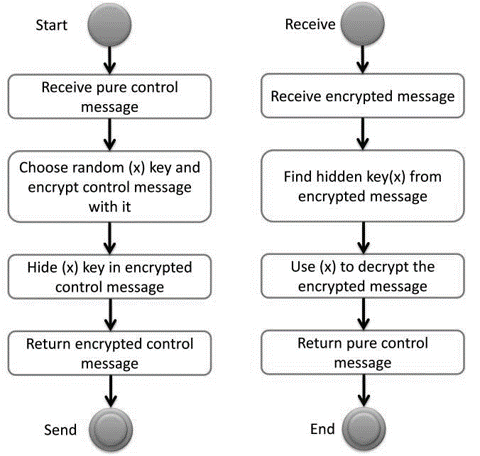
\includegraphics[scale=0.8]{gix.png}
\caption{GIX Algorithm}
\end{figure}
